% !TeX root = main.tex

\section{Q2: Relating Matrices and RANSAC}

\paragraph*{Question}
\begin{displayquote}
    % Contents of question 2
Describe and derive the Fundamental Matrix, Essential Matrix, and Homography Matrix (for the case of pure rotation). When there are many correspondences between two images, can these methods be used to filter out the best correspondences?

\end{displayquote}

Before answering the questions, it is essential to brief on Epipolar Geometry.

\subsection{Epipolar Geometry}

Consider the image below where two cameras are capturing the images of the world.

\begin{figure}[h]
    \centering
    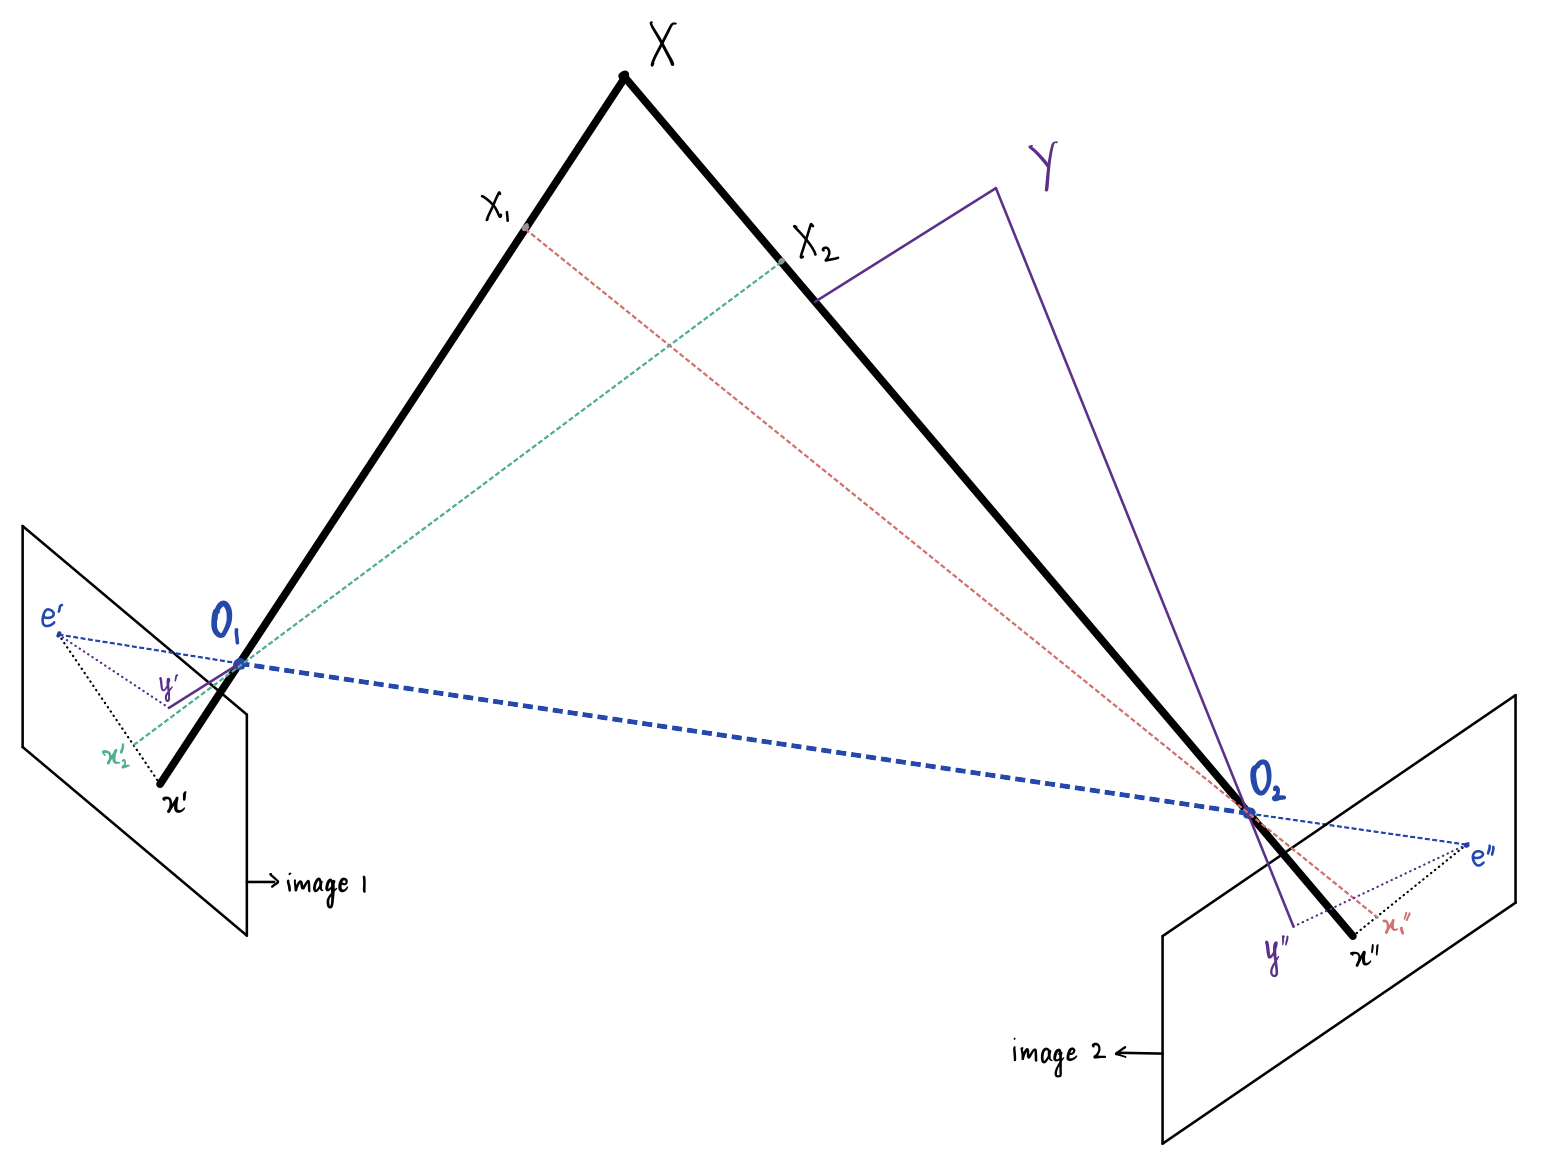
\includegraphics[width=0.75 \textwidth]{Epipolar_geometry.PNG}
    \caption{Epipolar Geometry}
    \label{fig:q2-epipolar-geometry}
    \small
        Points $X$ and $Y$ are points in the real world whose image falls at (pixel locations) $x'$ and $y'$ in image 1 and $x''$ and $y''$ in image 2. 
        The origins of these cameras are located at $O_1$ and $O_2$, respectively.

        As a convention, points in the first image have a single hyphen, whereas points in the second image have two hyphens.
\end{figure}

\paragraph*{Epipolar Axis}
The line joining $O_1$ and $O_2$ is called the \textbf{epipolar axis}. It intersects the images at $e'$ and $e''$ respectively.

\paragraph*{Epipolar Plane}
We know $O_1 O_2 X$ form a plane (they are three points in the world). This plane is called the \textbf{epipolar plane}.

\paragraph*{Epipolar Line}
It is clear that the image of $X_1$ in camera 1 will also fall on $x'$ (same line), similarly the image of $X_2$ in camera 2 will also fall on $x''$. However, the image of $X_1$ in camera 2 will fall at $x_1''$, which is on the line joining $x''$ and $e''$. This line is called the \textbf{epipolar line}. Similarly, the image of $X_2$ in camera 1 will fall at $x_2'$ (which is also on the line joining $e'$ and $x'$).

When $X_1$ moves along $\overline{XO_1}$, its image $x''_1$ traces a line in the second image (the \textit{epoipolar line}). Same can be said for $X_2$ and the first image.

% Fundamental Matrix
\subfile{q2_v1_fmat.tex}

% Essential Matrix
\subfile{q2_v1_emat.tex}

% Rotation Homography
\subfile{q2_v1_rhom.tex}

% RANSAC
\subfile{q2_v1_ransac.tex}
